%%%%%%%%%%%%%%%%%%%%%%%%%%%%%%%%%%%%%%%%%
% Design based on a template by Roberto and following the format of
% the xmipp tutorials. In turn, they seem to be based on a template
% from http://www.latextemplates.com
%%%%%%%%%%%%%%%%%%%%%%%%%%%%%%%%%%%%%%%%%

%----------------------------------------------------------------------------------------
%	PACKAGES AND OTHER DOCUMENT CONFIGURATIONS
%----------------------------------------------------------------------------------------

\documentclass[12pt]{article} % Default font size is 12pt, it can be changed here
\usepackage[english]{babel}
\usepackage[utf8]{inputenc}
\usepackage{listings} % To include source code
\usepackage{caption}
\usepackage{geometry} % Required to change the page size to A4
%\geometry{a4paper} % Set the page size to be A4 as opposed to the default US Letter
\usepackage{framed}
\usepackage{url}
\usepackage{graphicx} % Required for including pictures
\usepackage{natbib}
\usepackage{float} % Allows putting an [H] in \begin{figure} to specify the exact location of the figure
\usepackage{hyperref}
\usepackage{menukeys}

\usepackage{fancyhdr}
\pagestyle{fancy}
\fancyhf{}
\fancyhead[RO]{{Initial Volume Estimation Tutorial}} 
\fancyhead[LO]{Scipion}

%\fancyhead[RO]{{\leftmark}} 
\fancyfoot[LE,RO]{{ \thepage }}

%\usepackage{lipsum} % Used for inserting dummy 'Lorem ipsum' text into the template
\definecolor{grey}{rgb}{0.9,0.9,0.9}


\linespread{1.2} % Line spacing

%\setlength\parindent{0pt} % Uncomment to remove all indentation from paragraphs

\newcommand{\scipion}{\textsc{Scipion} }
\newenvironment{command}{\tt\begin{quote}}{\end{quote}}
\newcommand{\comm}[1]{\texttt{#1}}

\begin{document}

%----------------------------------------------------------------------------------------
%	TITLE PAGE
%----------------------------------------------------------------------------------------

\begin{titlepage}


% New command for horizontal lines. Change thickness here.
\newcommand{\HRule}{\rule{\linewidth}{0.5mm}}

\center % Center everything on the page


\includegraphics{../tutorial_common/images/scipion_logo.png}

{\large Scipion Tutorial Series}\\[1.0cm]

\textsc{\LARGE National Center for Biotechnology}\\[0.5cm]
\textsc{\Large Biocomputing Unit}\\[0.5cm]

\HRule\\[0.4cm]
{ \huge \bfseries Initial Volume Estimation Tutorial}\\[0.4cm] % Title of your document
\HRule \\[1.5cm]

%{\large \today}\\[3cm] % Date, change the \today to a set date if you want to be precise

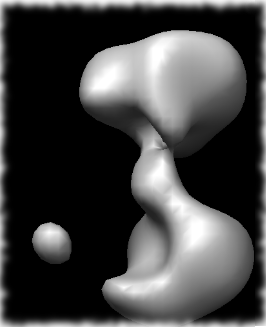
\includegraphics[width=0.35\textwidth]{{images/00.ReconstructedVolume}.png}

\vfill % Fill the rest of the page with whitespace
%\begin{minipage}{0.4\textwidth}
\begin{flushright}
 \large
%\emph{Author:}\\
  \textsc{Scipion Team} % Your name
\end{flushright}
%\end{minipage}

\end{titlepage}


%----------------------------------------------------------------------------------------
%	OBJETIVOS
%----------------------------------------------------------------------------------------



\subsection*{Intended audience}

This tutorial is an introduction to the estimation of an initial
volume using Scipion.  Only a very limited knowledge about 3D-EM image
processing and Scipion is required, and basic computer skills.

\subsection*{We'd like to hear from you}

We have tested and verified the different steps described in this demo
to the best of our knowledge, but since our programs are in continuous
development you may find inaccuracies and errors in this text. Please,
let us know about any error you find, as well as your suggestions for
future editions by writing to
\href{mailto:scipion@cnb.csic.es}{scipion@cnb.csic.es}.

\newpage

%----------------------------------------------------------------------------------------
%	TABLE OF CONTENTS
%----------------------------------------------------------------------------------------

\tableofcontents % Include a table of contents

\newpage % Begins the essay on a new page instead of on the same page as the table of contents 


\section{General Introduction}

\subsection{Initial Volume Estimation}

Single Particle Analysis (SPA) techniques are used to obtain 3D maps
of biological complexes at near-atomic resolution. They do so by
combining tens of thousands of projection images obtained by
Transmission Electron Microscopy (TEM). In general, the reconstruction
process that leads to the final 3D map requires the use of an
approximate low resolution initial model, to be refined in further
steps.

In this tutorial we present different methods to obtain this initial
model using Scipion: Xmipp Random Conical Tilt, Xmipp 3D-RANSAC and
Eman Initial Model.

\section{Software Installation}

The first step is to download and install \scipion and related
software packages. We describe briefly the process in the next
sections. For the full documentation please refer to
\url{http://scipionwiki.cnb.csic.es/bin/view/TWiki/NewInstallation}.

\subsection{Xmipp}

One of the main components of \scipion is the Xmipp package. To get
the latest version use:

\begin{command}
git clone http://git.code.sf.net/p/newxmipp/code xmipp
\end{command}

\noindent
then change to the \directory{xmipp} directory and run the installation with

\begin{command}
./install.sh
\end{command}

\subsection{Scipion}

To get the latest version of \scipion run

\begin{command}
git clone http://git.code.sf.net/p/pyworkflow/code scipion
\end{command}

\noindent
and then change into the \directory{scipion} directory. Finally run:

\begin{command}
./scipion install --with-all-packages --with-xmipp=\$XMIPP\_HOME
\end{command}

\noindent
where \verb+$XMIPP_HOME+ points to the directory with your local
installation of Xmipp.

\subsection{Sample Data}

To download the data you will work with, use the following command:

\begin{command}
scipion testdata --download rct
\end{command}

It will be downloaded in \verb+$SCIPION_HOME/data/tests/rct+.

Afterwards, you can launch the main GUI by typing:
\verb+scipion+. Create a new project by clicking on the \keys{Create
  Project} button, type a \textit{project name} and click on
\keys{OK}. This will create a new project window.

\section{Xmipp Random Conical Tilt}

One of the most widespread SPA techniques is the Random Conical Tilt (RCT) \citep{Radermacher1987a}.
In RCT the assumption is that we have a randomly distributed particle in all its conformations and positions
along a sample, so when we take a low-power image, we are getting multiple views of the same particle.
The specimen stage of the microscope is then tilted and a new low-power image is taken.

The less power is used, the less exposure of the sample. Having a low
exposure is a cryoEM constraint on biological objects.  As a result,
we get images with low signal-to-noise ratio (SNR). With these two
images, every processing program will need to relate each particle to
its tilted version in order to get different views of the specimen and
estimate the tilt angle.

\begin{figure}
\centering
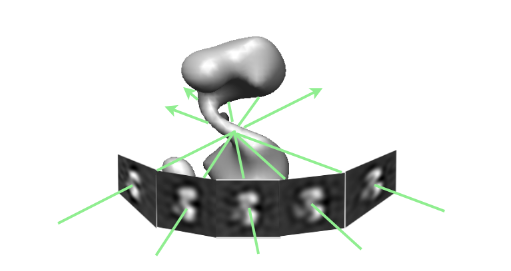
\includegraphics[width=0.75\textwidth]
{{images/01.RCTprojection}.png}
\caption{How the projections vary with the tilt.}
\label{RCTprojection}
\end{figure}

\subsection{Importing Tilted Pairs of Micrographs}

Go to the \keys{View} selection menu on the top left panel and select
\textbf{Random Conical Tilt}.

The first step is to import the tilted pairs of micrographs to your
scipion project. To do this, select the \menu{Import micrograph pairs}
protocol. In \textit{Pattern untilted} and \textit{Pattern tilted} we
have to indicate where the untilted and tilted micrograph files are
stored (to do so you can click on the \keys{browse} button next to the
text entries, the one that looks like a folder).

The complete patterns are:

\begin{verbatim}
$SCIPION_HOME/data/tests/rct/micrographs/F_rct_u_*.tif
$SCIPION_HOME/data/tests/rct/micrographs/F_rct_t_*.tif
\end{verbatim}

%In this first version pairs assignment is done by micrograph order but in next versions a wizard
%will be provided.

Modify the parameters of the Import Micrographs protocol according to
the ones shown in figure \ref{ImportMics}. When you have completed the
form, click on the \keys{Execute} button.

\begin{figure}[H]
\centering
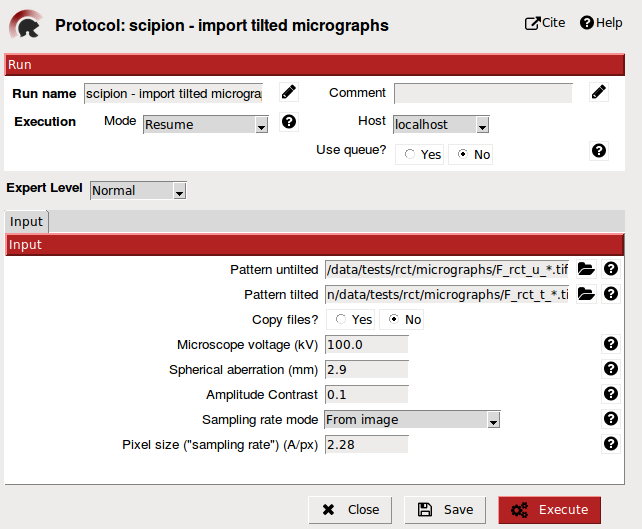
\includegraphics[width=0.75\textwidth]
{{images/02.ImportMics}.png}
\caption{Dialog of the Import Micrographs protocol.}
\label{ImportMics}
\end{figure}

Once the protocol has finished you can press on the \keys{Analyze
  Results} button and a new window will open where you can see the
imported micrograph pairs, as shown in figure \ref{ImportResults}.

\begin{figure}
\centering
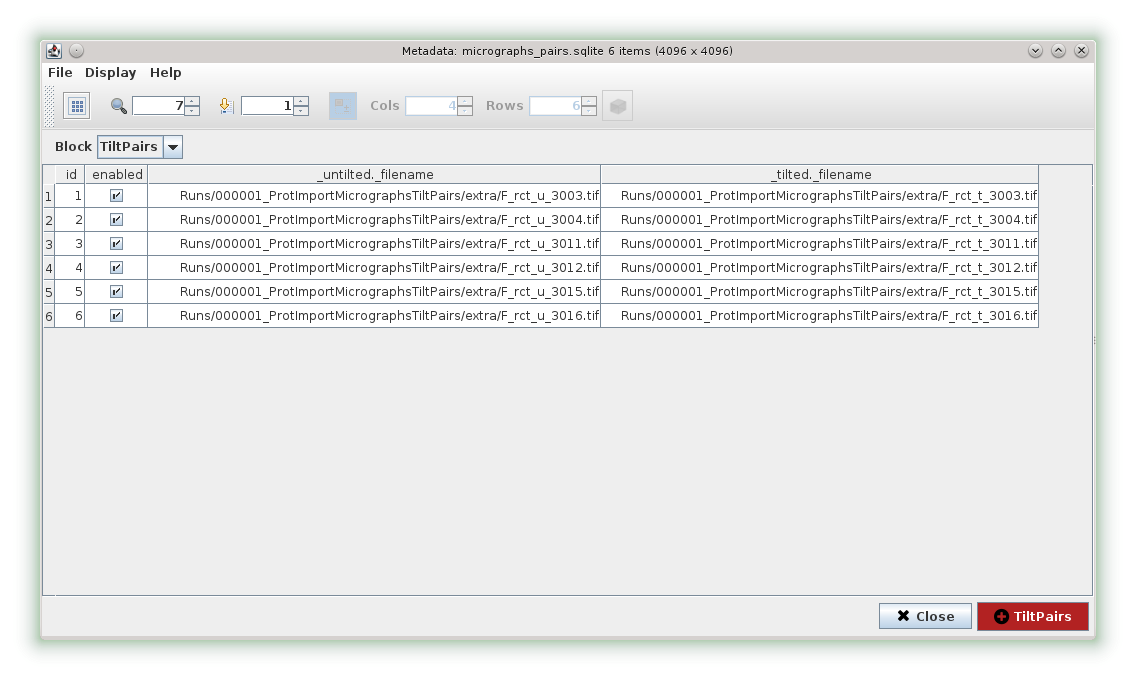
\includegraphics[width=0.75\textwidth]
{{images/03.ImportResults}.png}
\caption{Visualizing the Import Micrographs results.}
\label{ImportResults}
\end{figure}

\subsection{Particle Picking}

After we import the micrographs we need to pick tilted and untilted particle pairs.

Go to the \menu{Picking micrograph pairs} protocol and double-click on
it. A form as the one shown in figure~\ref{PickingProtocol1} will
appear. Select the Micrographs Tilt Pair object produced by the import
protocol as input (see figure~\ref{PickingProtocol2}) and click on the
\keys{Execute} button. This will open the Xmipp particle picking GUI.

\begin{figure}[H]
\centering
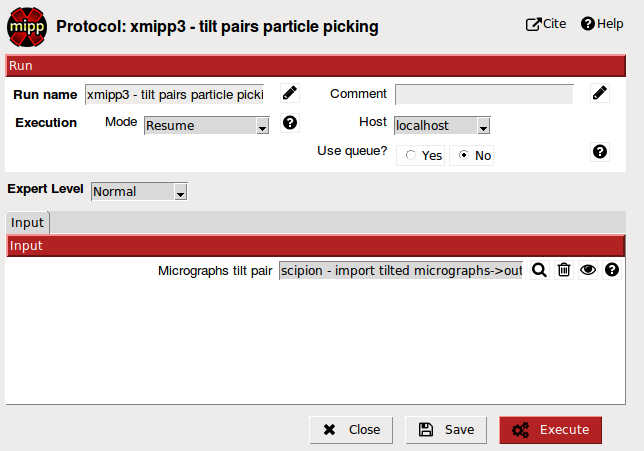
\includegraphics[width=0.75\textwidth]{{images/04.PickingProtocol1}.png}
\caption{Picking pairs protocol.}
\label{PickingProtocol1}
\end{figure}

\begin{figure}
\centering
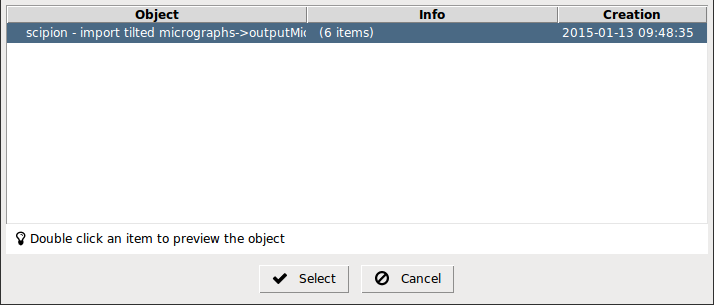
\includegraphics[width=0.75\textwidth]{{images/04.PickingProtocol2}.png}
\caption{Selection of the imported micrographs in the Picking pairs protocol.}
\label{PickingProtocol2}
\end{figure}

If you find the particles difficult to see due to noise and the
contrast of the images, you can use the different filters on the
\menu{Filters} menu, on the top of the Xmipp Til Pair Picker dialog.
For instance you might select the \menu{Filters > Brightness/Contrast}
filter and press the \keys{Auto} button that will set the brightness
and contrast to the optimal values for the selected micrograph. Then
change to other micrograph and do the same. The resulting images will
be much easier to use for picking.

We will explain shortly how to use a shortcut to avoid the
time-consuming picking of the particles in this tutorial, but if you
want to do the actual picking, these are the steps:

\begin{enumerate}

\item Find the first particle in both the untilted and tilted
  micrographs. This can be tricky, try to find a common reference in
  the micrographs. Then pick first the untilted and then its tilted
  pair. Note that zooming in or out can help. To zoom in, press
  \keys{shift} and scroll up, to zoom out, press \keys{shift} and
  scroll down.

\item Pick three more particles like the first one. From this point,
  the program will propose the tilted pair position for each new
  selected particle. You can correct the guessed position of the
  tilted one, and it is important to do it, so the tilt estimation can
  be properly set. During the picking of the first particles the
  manual error correction will help the algorithm to learn and propose
  a better tilt adjustment. For correcting the errors, it is normally
  better to zoom in the micrograph.

\item Finally continue picking just the untilted (tilted will
  automatically be picked) but keeping an eye on the tilted, in order
  to prevent deviations due to accumulated errors. The amount of
  particles to pick for a good reconstruction varies depending on the
  tilt angle, the quality of the micrographs and many other factors,
  but a good starting point could be 2000 particles.

\end{enumerate}

However if you don't feel like picking manually thousands of particles
you can import the already picked particles by clicking on \menu{File
  > Import coordinates} as shown on figure~\ref{PickingGUI}, and
specifying the following path:

\begin{verbatim}
$SCIPION_HOME/data/tests/rct/positions
\end{verbatim}

\begin{figure}[H]
\centering
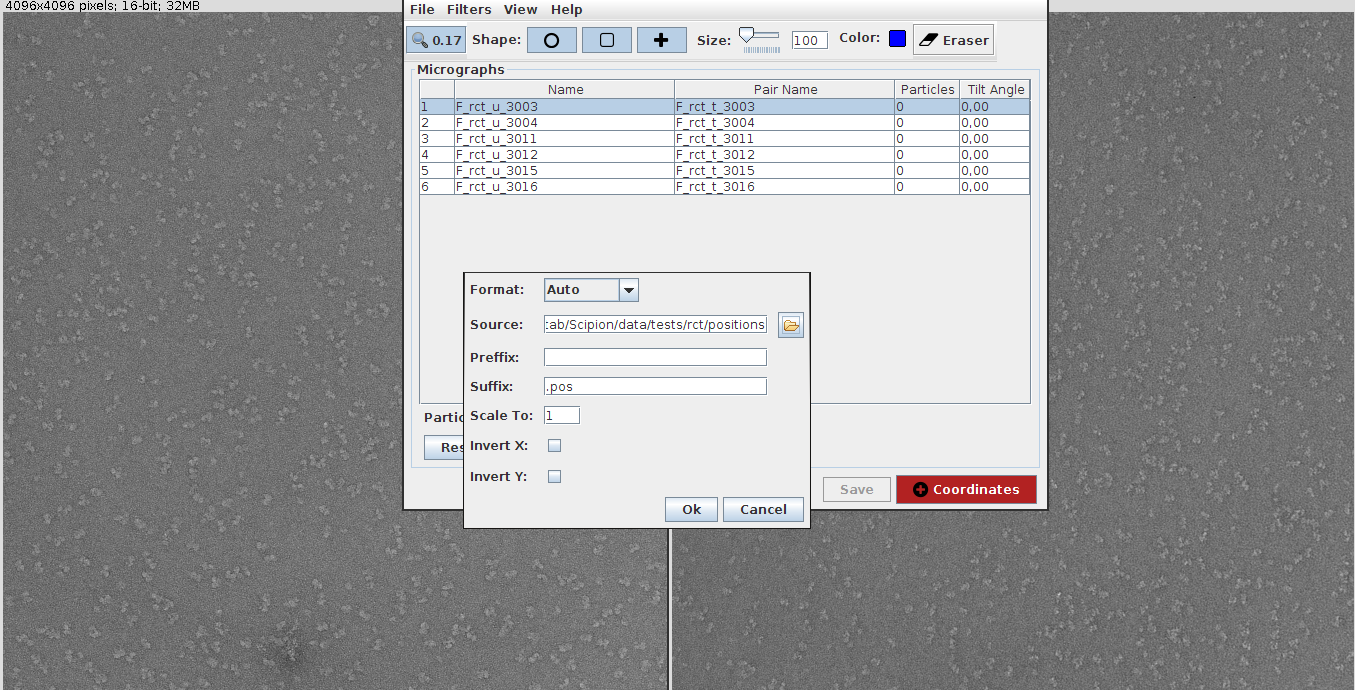
\includegraphics[width=0.75\textwidth]{{images/05.PickingGUI}.png}
\caption{Xmipp particle picking pairs GUI.}
\label{PickingGUI}
\end{figure}

Notice that after running the protocol, its status will not change to
\textbf{Finished} but will remain as \textbf{Interactive}.  This
allows us to execute it again if we wish to pick more particles.

\subsection{Extraction of Particle Pairs}

Now that we have picked coordinate pairs, they have to be extracted as
particle pairs.  To do so select the \menu{Extract particle pairs}
protocol and fill in the parameters as shown in
figure~\ref{ExtractPairs}.  Although particles were picked with a size
of 120 pixels, we will downsample them by a factor of 2 in the
extraction to speed up the next steps.

Once the protocol has finished you can review the particles by
clicking on the \keys{Analyze Results} button as seen in
figure~\ref{ExtractResults}.
%If you don't like some of the particles you can disable them and create a subset with the good ones. Just click on the \textbf{TiltPairs} red button and give the subset a name.

\begin{figure}
\centering
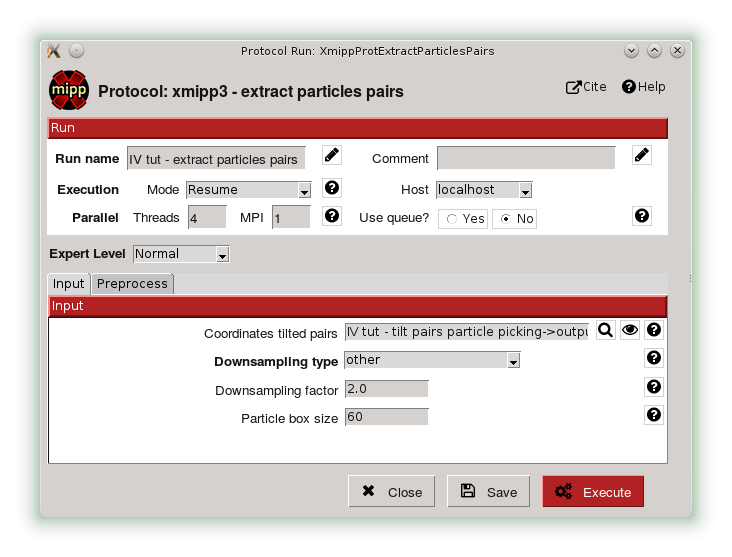
\includegraphics[width=0.75\textwidth]{{images/06.ExtractPairsProtocol}.png}
\caption{Extract particle pairs protocol.}
\label{ExtractPairs}
\end{figure}

\begin{figure}[H]
\centering
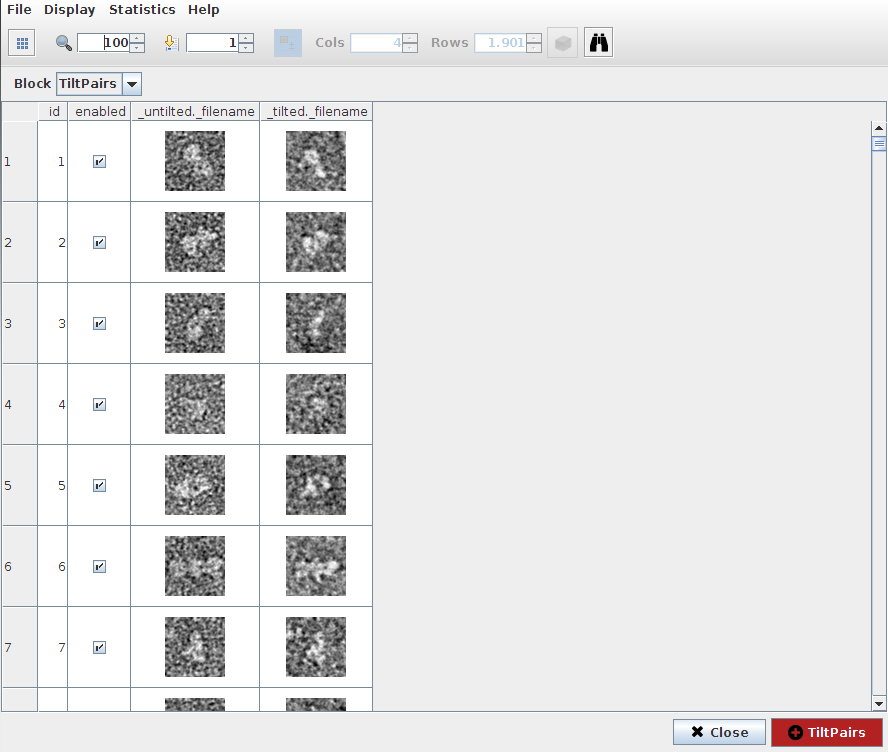
\includegraphics[width=0.75\textwidth]{{images/07.ExtractPairsResults}.png}
\caption{Extract particle pairs results.}
\label{ExtractResults}
\end{figure}

\subsection{Classification with Xmipp CL2D}

Once we have extracted the particles, they have to be classified in
order to group those belonging to different states of the particle, or
even to find those that come from an error in the picking.


For this tutorial we will perform a CL2D classification with Xmipp,
but we could choose any of the other 2D classification protocols
available. Go to the \keys{View} selection menu on the top left panel
and select \textbf{Protocols SPA}. Then select \menu{2D > Classify >
  xmipp3 - cl2d}.

For the \textit{Input images} select the set of untilted particles
produced in the previous step, fill in the rest of the parameters as
shown in figure~\ref{CL2D} and press \keys{Execute}.

\begin{figure}
\centering
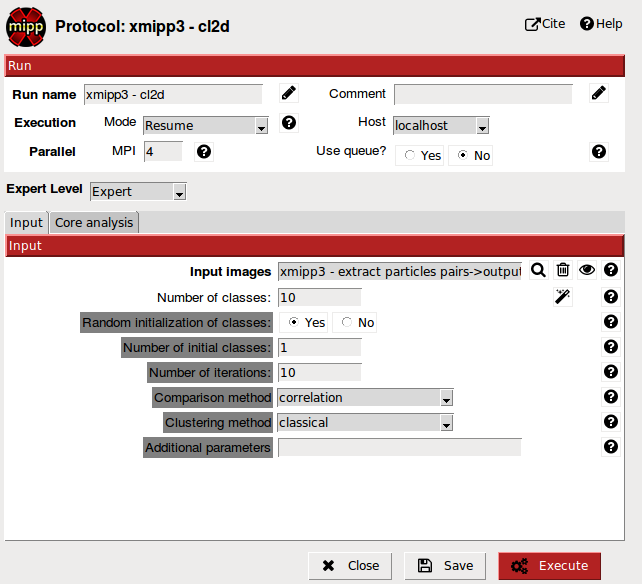
\includegraphics[width=0.65\textwidth]{{images/08.CL2Dprotocol}.png}
\caption{CL2D protocol.}
\label{CL2D}
\end{figure}

This protocol will take some time to finish (depending on your
computer power and the number of \textbf{MPI}s chosen).  Once it has
finished we can visualize the classes obtained by clicking on
\keys{Analyze Results}.

These classes show averaged images that represent our particles. But
to be sure that they are representing them with fidelity, we need at
least some basic checks:

\begin{itemize}
  
\item We should be using the stable core classes. These are composed
  by those particles that have stayed through all iterations together.

\item Each class should contain between 100 and 200 particles more or
  less. Less than that will result in reconstructions of low quality,
  so the estimation is not being properly done. Also, more than
  200-250 particles would result in a wrong estimation because very
  different particles could be appearing in the same class.

\end{itemize}

Apart from that, there is also a subjective assessment, and it comes
from what the user is looking for.  Each class shows an average image
that can give you an idea of what we would find if we start a
reconstruction with those images.  The user must select those volumes
that are more promising. In our case, classes 3 and 7 have been
discarded, because they seem to show particles in a top view (or just
one part of the particle).

%Then, as done with particles extracted, you should create a subset of classes to be used as input for next step, 
%as shown in figure~\ref{CL2Dresults}
Finally we will create a subset of classes to be used as input for the
next step, as shown in figure~\ref{CL2Dresults}.

\begin{figure}[H]
\centering
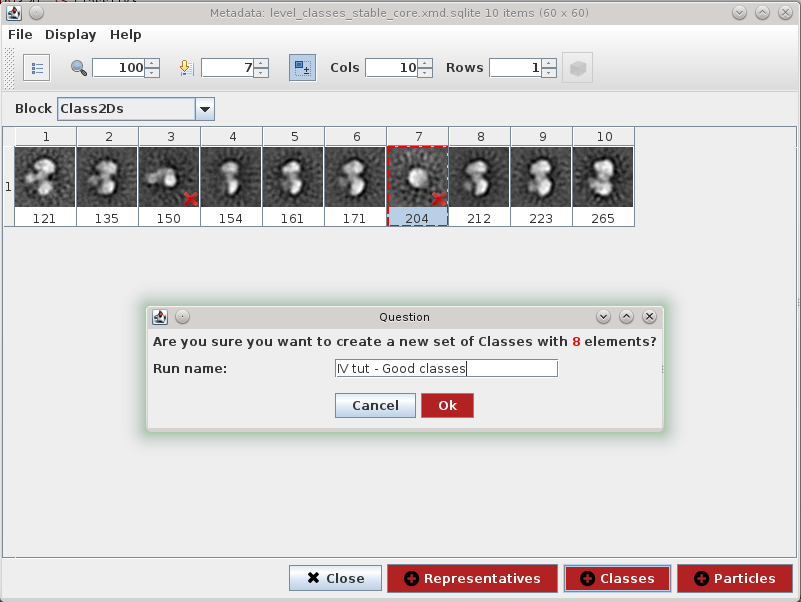
\includegraphics[width=0.65\textwidth]{{images/09.GoodClasses}.png}
\caption{CL2D results.}
\label{CL2Dresults}
\end{figure}

\subsection{Initial Volume Generation with Random Conical Tilt}

Now that you have the desired classes, only the RCT reconstruction step is left. 

Select protocol \textbf{Random Conical Tilt} and fill in the form as shown in figure~\ref{RCTprotocol}.

You have to provide the particles tilt pair object produced by the extraction (or a subset) and the particles or classes 
you want to reconstruct. Take into account that if you choose particles they should contain alignment information.
The \textbf{Thin Object} option must be set to “Yes” if the particle is not more or less spherical. 
When the object is going to change its width significantly between the untilted and the tilted image, we can considered this a “thin object”. 
Reconstruction can also low-pass filter the volumes after the process is done, producing both filtered and not filtered volumes as output.

In order to visualize the volumes click on \keys{Analyze results} after the protocol has finished, and a window as the one on figure~\ref{RCTresults} 
will show up.

\begin{figure}[H]
\centering
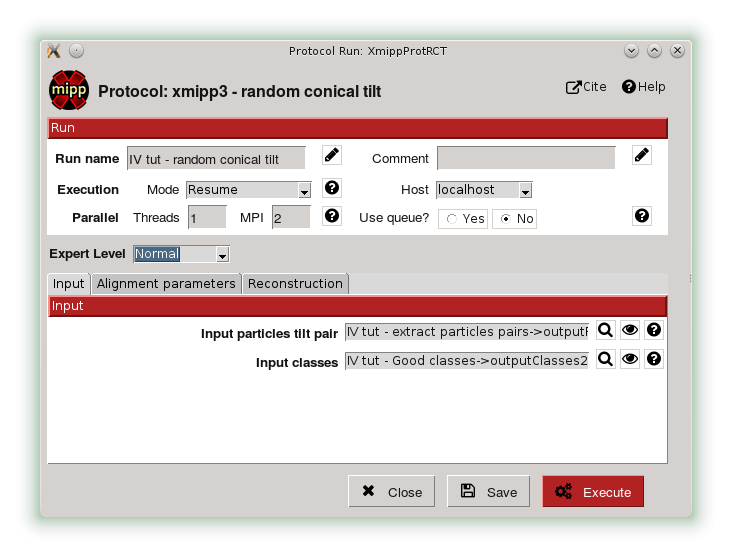
\includegraphics[width=0.6\textwidth]{{images/10.RCTprotocol}.png}
\caption{Xmipp RCT protocol}
\label{RCTprotocol}
\end{figure}

\begin{figure}
\centering
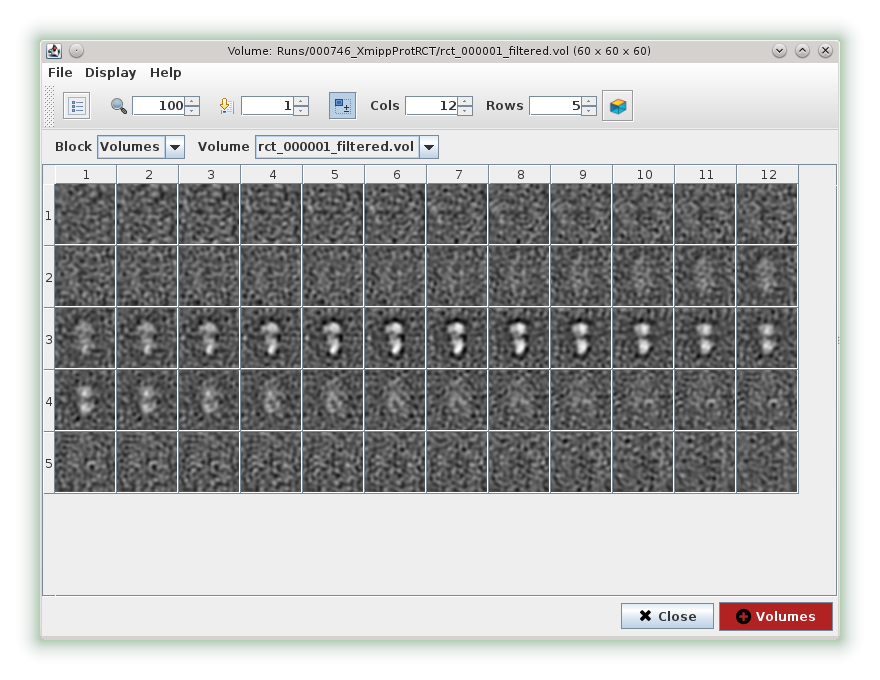
\includegraphics[width=0.6\textwidth]{{images/11.RCTresults}.png}
\caption{Xmipp RCT output: Filtered volume.}
\label{RCTresults}
\end{figure}

\section{3D Ransac}

In this section, we present how to use Xmipp 3D-RANSAC approach, which can obtain a reliable low resolution initial volume 
from sets of macromolecular projection images without a priori information ( Vargas et al. (2014)). 

\subsection{Initial Volume Generation with 3D Ransac}

Change to the \textbf{Protocols SPA} view if you are not already there, go to \menu{3D > Initial Volume > xmipp - ransac} protocol. 

As input we will use the classes obtained on Random Conical Tilt section so we can compare the generated volumes using different 
techniques. Also, fill in the other form parameters as shown in figure~\ref{RansacProtocol} and explained below. 

\begin{figure}
\centering
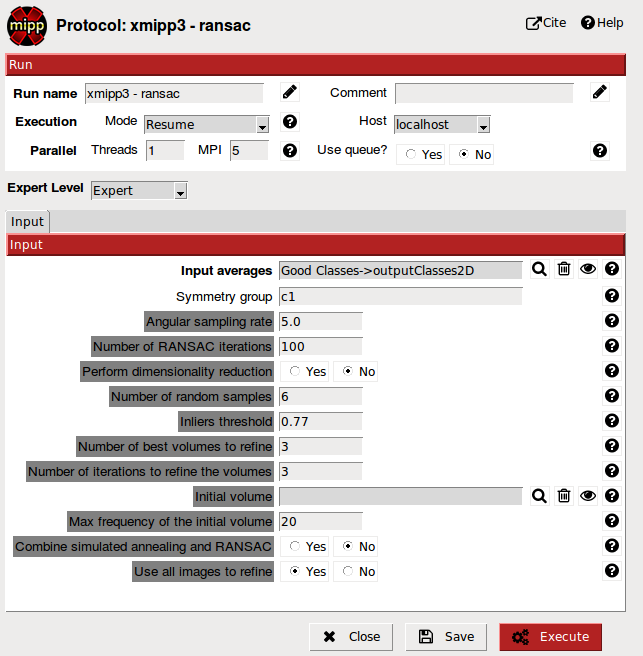
\includegraphics[width=0.75\textwidth]{{images/15.RansacProtocol}.png}
\caption{Xmipp Ransac protocol.}
\label{RansacProtocol}
\end{figure}

There is not symmetry so leave c1 and the angular sampling, in degrees, defines how fine the projection gallery from the volume is explored. 
The number of RANSAC iterations are the number of random volumes which are generated, in our case 100. 
We select performing dimensionality reduction, with a number of grids per dimension equal to 6, and therefore each
random volume is generated from 36 (6x6) classes. 
The inlier threshold is a correlation based cutoff to determine if a class is an inlier of the generated random volume or not. 
Note that in cases where the classes have very low noise this value must be increased ( 0.8-0.95) and, on the other hand, 
in cases with high noise, this value must be decreased. 
The \textbf{Number of best volumes to refine} are the number of volumes, among all the generated ones (in this case 100), that
are going to be further refined using a projection matching approach by the selected \textbf{Number of iterations to perform to refine the volumes}. 
Finally, \textbf{Max frequency of the initial volume} is the maximum frequency of the initial volume in Angstroms. 
Press the \keys{Execute} button and wait until the protocol has finished when output volumes could be visualize by clicking 
on \keys{Analyze Results} button as seen in figure~\ref{RansacResults}

\begin{figure}
\centering
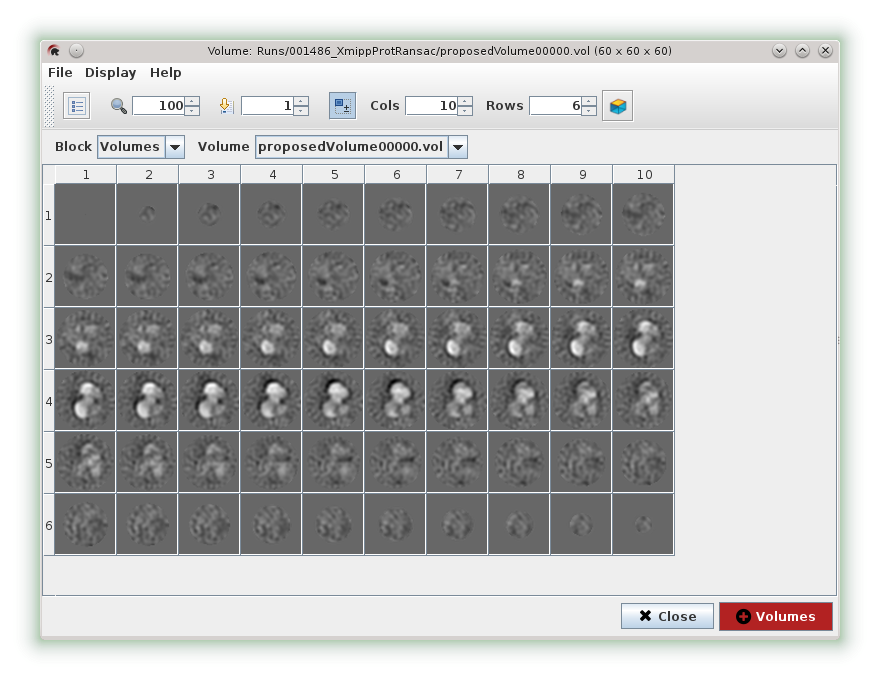
\includegraphics[width=0.75\textwidth]{{images/16.RansacResults}.png}
\caption{Xmipp Ransac output volumes.}
\label{RansacResults}
\end{figure}

\newpage

\section{Eman initial model}

In this section we present how to obtain an initial module in Scipion using Eman initial model.

\subsection{Initial Volume Generation with Eman}

Change to the \textbf{Protocols SPA} view if you are not already
there, go to \menu{3D > Initial Volume > eman2 - initial model}
protocol.  As we did before use the classes obtained on Random Conical
Tilted section as input so we can compare the generated volumes using
different techniques. Also, fill in the other form parameters as shown
in figure~\ref{EmanProtocol}

Once the protocol has finished go and view the generated output volumes by clicking on \keys{Analyze results}, as you can see in figure~\ref{EmanResults}.

\begin{figure}[H]
\centering
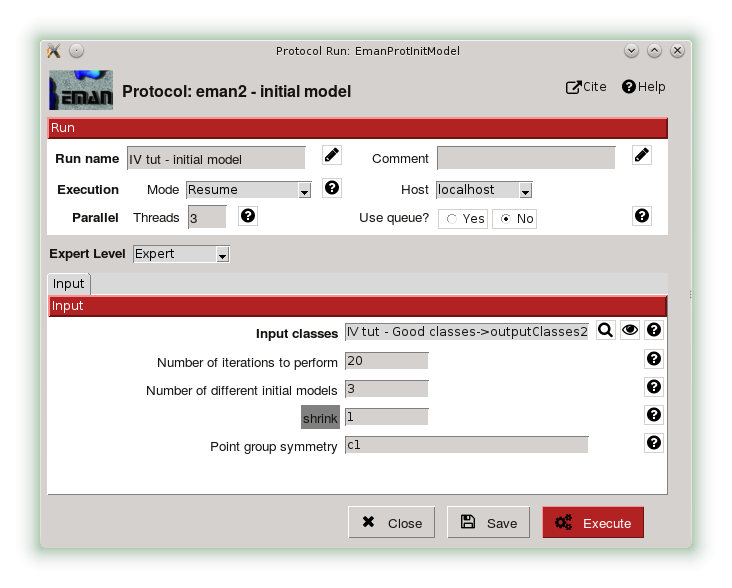
\includegraphics[width=0.75\textwidth]{{images/17.EmanProtocol}.png}
\caption{Eman protocol.}
\label{EmanProtocol}
\end{figure}

\begin{figure}
\centering
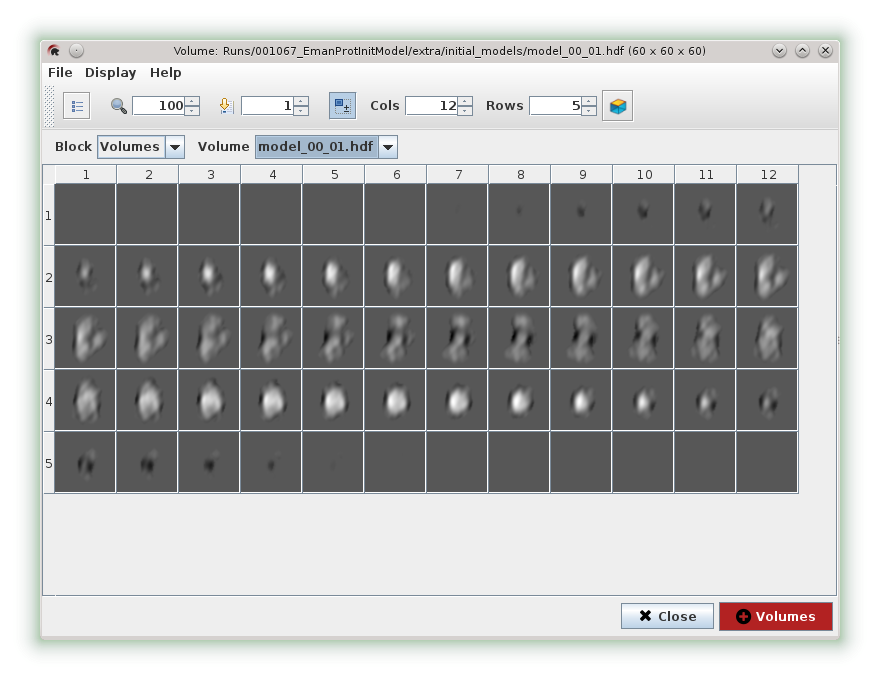
\includegraphics[width=0.75\textwidth]{{images/18.EmanResults}.png}
\caption{Eman generated output volumes.}
\label{EmanResults}
\end{figure}

\bibliographystyle{apalike}
\bibliography{../tutorial_common/em.bib}

\end{document}
